\documentclass{article}
\usepackage[utf8]{inputenc}
\usepackage{tikz}
\usetikzlibrary{shapes.geometric, arrows}
\renewcommand\familydefault{\sfdefault}

\tikzstyle{startstop} = [rectangle, rounded corners, text width=3cm, minimum width=3cm, minimum height=1cm,text centered, draw=black, fill=red!50]

\tikzstyle{io} = [trapezium, trapezium left angle=70, trapezium right angle=110, minimum width=3cm, minimum height=1cm, text centered, draw=black, fill=blue!50]

\tikzstyle{process} = [rectangle, text width=3cm, minimum width=3cm, minimum height=1cm, text centered, draw=black, fill=orange!70]

\tikzstyle{decision} = [diamond, text width=3cm, minimum width=3cm, minimum height=1cm, text centered, draw=black, fill=green!50]

\tikzstyle{arrow} = [thick,->,>=stealth]

\begin{document}
\pagenumbering{gobble}
\section*{Legend}

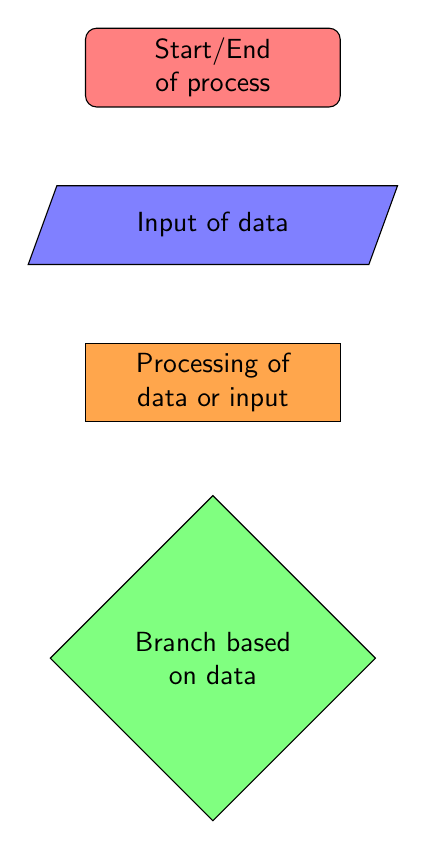
\begin{tikzpicture}[node distance=2cm]

\node [startstop] (start) {Start/End of process};
\node [io, below of= start] (io) {Input of data};
\node [process, below of=io] (process) {Processing of data or input};
\node [decision, yshift=-1.5cm, below of=process] (descision) {Branch based on data};

\end{tikzpicture}

\end{document}
